\problemname{Maze}

Filip (and his dad) started experimenting with robotics. They built a robot that moves through a maze drawn on a rectangular graph paper with some grid squares colored black. The robot's color sensor prevents it from going on or through the black regions---they act like walls. The graph paper is on a huge black board, guaranteeing that the robot stays on the paper. As for the robot's moves, it ``jumps'' from one grid square to one of the four adjacent grid squares (this required some very fine precision and they are justly proud of their work). There is only one problem: the robot stubbornly refuses to jump more than twice in a row in the same direction. It also refuses to jump backwards to the location it just came from (though it can revisit the same location later).

After watching the robot skip happily through the maze, Filip decided that it needed a destination. He colored one of the grid squares red and with dad's help reprogrammed the robot to start singing once it finds the red square.

Sometimes Filip needs to wait for the singing for a very long time since the robot usually meanders through the maze. In such cases, Filip wonders how long would it take to move along the shortest route. Naturally, you want to help him: compute the smallest number of steps the robot needs to make to get to the red square.

% variant 1: from the top left corner to the bottom right corner
% variant 2: how to extend exactly one of the lines so that the shortest path gets extended the most?
% variant 3: multiple dots

\section*{Input}
The first line contains $k$, the number of mazes.
Each maze is described on several lines. The first line is empty. The second line contains two integers $a$ and $b$, the dimensions of the graph paper. Then $a$ lines follow, each with a string of length $b$. The strings contain only symbols `.' corresponding to an uncolored grid square, `B' corresponding to a black square, `R' corresponding to the robot, or `D' corresponding to the destination (red square). You may assume that $a,b\leq$ 1,000 and that there is exactly one robot (standing on an uncolored square), and exactly one red square.


\section*{Output}
The output contains $k$ lines. The $i$-th line corresponds to the $i$-th maze.
It contains {\tt -1} if there is no route through the maze that leads to the red square.
Otherwise, it contains the smallest number of steps needed to get to the red square.


\section*{Note}
Shortest routes for the first three sample inputs are shown below. There is no route for the fourth sample input, shown on the right.
\begin{figure}[h]
  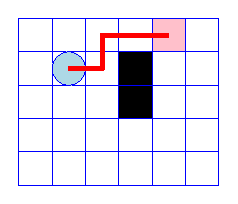
\includegraphics[scale=0.7]{maze1} \hskip 1cm
  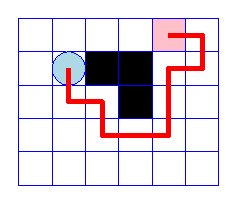
\includegraphics[scale=0.7]{maze2} \hskip 1cm
  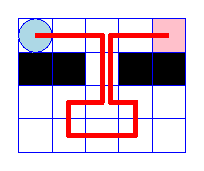
\includegraphics[scale=0.7]{maze3} \hskip 1cm
  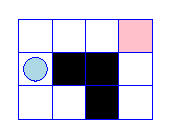
\includegraphics[scale=0.7]{maze4}
\end{figure}
